\subsection{Introduction}
\label{sub:introduction}
\begin{example}
    Un automate fini :
    \begin{itemize}[label=\textbullet]
        \item lit la séquence des lettres de gauche à droite.
        \item possède un nombre fini d'états.
        \item en fonction de la lettre courante et de la lettre lue, se déplace vers un autre état.
        \item possède un unique état initial ainsi que des états finaux.
        \item accepte un mot si et seulement s'il se termine sur un état final.
    \end{itemize}
    \begin{figure}[H]
        \centering
        \begin{tikzpicture} [node distance = 3cm, 
            on grid, 
            auto,
            every loop/.style={stealth-}]
        
        % State q0 
        \node (q0) [state, 
            initial, 
            accepting, 
            initial text = {}] {$q_0$};
        
        % State q1    
        \node (q1) [state,
            right = of q0] {$q_1$};
        
        % Arrows
        \path [-stealth, thick]
            (q0) edge[bend left] node {$a$}   (q1)
            (q1) edge[bend left] node {$a$}   (q0)
            (q0) edge [loop above]  node {b}()
            (q1) edge [loop above]  node {b}();
        \end{tikzpicture}
        \caption{Exemple d'automate fini}
    \end{figure}
\end{example}

\subsection{Définitions et exemples}
\label{sub:definitions_et_exemples}

\begin{definition}{Langage}{langage}
    \begin{itemize}[label=\textbullet]
        \item un alphabet est un ensemble fini, que l'on note $\Sigma$.
        \item ses éléments sont appelés lettres ou symboles.
        \item un mot est une suite de symboles, $\epsilon$ est le mot vide.
        \item l'ensemble des mots sur $\Sigma$ est noté $\Sigma^*$.
        \item un langage est un sous-ensemble de $\Sigma^*$. ($L \subseteq \Sigma^*$)
    \end{itemize}
\end{definition}
\begin{definition}{Automate fini}{automate_fini}
    Un automate fini $A$ sur un alphabet $\Sigma$ est un 4-uplet $(Q, q_0, F, \delta)$ où :
    \begin{itemize}[label=\textbullet]
        \item $Q$ est un ensemble fini d'états.
        \item $q_0 \in Q$ est l'état initial.
        \item $F \subseteq Q$ est l'ensemble des états finaux.
        \item $\delta : Q \times \Sigma \rightarrow Q$ est la \textbf{fonction} de transition.
    \end{itemize}
\end{definition}
\begin{definition}{Exécution}{exécution}
    Une exécution d'un automate $A$ est une suite finie $e = q_0\sigma_1 q_1\sigma_2 ... \sigma_n q_n(n\geq 0)$ telle que :
    \begin{itemize}[label=\textbullet]
        \item $\forall i \in \{0, ..., n\}, q_i \in Q$.
        \item $\forall i \in \{1, ..., n\}, \sigma_i \in \Sigma$.
        \item $\forall i \in \{0, ..., n-1\}, \delta(q_i, \sigma_{i+1}) = q_{i+1}$.
    \end{itemize}
    Une exéution $e$ est dite \textbf{acceptante} si $q_n \in F$.
\end{definition}
\begin{definition}{Langage accepté}{langage_accepté}
    Le langage accepté par un automate $A$ (noté $L(A)$) est l'ensemble des mots pour lesquels il existe une exécution
    acceptante de $A$.
    \begin{equation*}
        L(A) = \{w \in \Sigma^* | \exists e \text{ exécution acceptante de } A \text{ sur } w\}
    \end{equation*}
\end{definition}
\begin{example}
    Pour $\Sigma = \{0,1\} :$
    \begin{figure}[H]
        \centering
        \begin{tikzpicture} [node distance = 3cm, 
            on grid, 
            auto,
            every loop/.style={stealth-}]
        
        % State q0 
        \node (q0) [state, 
            initial,  
            initial text = {}] {$q_0$};
        
        % State q1    
        \node (q1) [state,
            right = of q0] {$q_1$};

        % State q2
        \node (q2) [state,
            right = of q1] {$q_2$};

        % State q3
        \node (q3) [state,
            accepting,
            right = of q2] {$q_3$};

        
        % Arrows
        \path [-stealth, thick]
            (q0) edge node {1}   (q1)
            (q1) edge node {0}   (q2)
            (q2) edge node {1}   (q3)
            (q2) edge [bend left] node {0} (q0)
            (q0) edge [loop above]  node {0}()
            (q1) edge [loop above]  node {1}()
            (q3) edge [loop above]  node {0,1}();
        \end{tikzpicture}
    \end{figure}
    Le langage accepté par cet automate est :
    \begin{equation*}
        L(A) = \{w\in \{0,1\}^* | w \text{ contient le facteur } 101\}
    \end{equation*}
\end{example}
\begin{definition}{Automate Complet}{automate_complet}
    Un automate $A$ est dit \textit{complet} si sa fonction de transition est totale.
\end{definition}
\begin{lemma}{Transformation d'un automate en un automate complet}{transformation_automate_complet}
    On peut toujours transformer un automate $A$ en un automate $B$ complet qui accepte le même langage, tel que $L(A) = L(B)$.  
\end{lemma}
\begin{remark}
    Effectivement, il \textit{suffit} de rajouter un état supplémentaire (état puit) non final et ajouter les transitions 
    manquantes vers cet état.
\end{remark}



\subsubsection{Test du vide}
Le problème du vide est le suivant :
\begin{itemize}
    \item Entrée $\Rightarrow$ Étant donné un automate $A$ sur un alphabet $\Sigma$.
    \item Sortie $\Rightarrow$ est-ce que $L(A) = \emptyset$ ?
\end{itemize}
\begin{definition}{Etats atteignables}{états_atteignables}
    Soit $A=(Q, q_0, F, \delta)$ un automate sur un alphabet $\Sigma$. Un état $q\in Q$ est dit \textit{atteignable} si 
    il existe un mot $w\in \Sigma^*$ et une exécution de $A$ sur $w$ qui termine en $q$.
\end{definition}
\begin{remark}
    L'ensemble des états atteignables d'un automate peut être calculé en temps $O(n+m)$, où $n$ est le nombre d'états et
    $m$ le nombre de transitions.
\end{remark}
\begin{theorem}{Test du vide}{test_vide}
    Étant donné un automate $A$ avec $n$ états et $m$ transitions, on peut tester en temps $O(n+m)$ si $L(A) = \emptyset$.
\end{theorem}
L'algorithme serait le suivant :
\begin{enumerate}
    \item Calculer l'ensemble des états atteignables $R$ de $A$.
    \item tester si $R \cap F = \emptyset$.
\end{enumerate}



\subsubsection{Opérations Booléennes}
\begin{definition}{Complément}{complément}
    Le complément d'un langage $L\subseteq \Sigma^*$ est le langage, noté $\overline{L}$, défini par :
    \begin{equation*}
        \overline{L} = \{w\in \Sigma^*|w\notin L\} = \Sigma^* \setminus L
    \end{equation*}
\end{definition}
\begin{example}
    Si $L$ est l'ensemble des mots sur $\{a,b\}$ qui contiennent au moins un $a$, alors $\overline{L}$ est l'ensemble des
    mots qui contiennet au moins deux $a$, ou pas de $a$.
\end{example}
\begin{definition}{Union et intersection}{union_intersection}
    Soient $L_1, L_2 \subseteq \Sigma^*$ deux langages. L'union et l'intersection de $L_1$ et $L_2$ sont définies par :
    \begin{equation*}
        L_1 \cup L_2 = \{w\in \Sigma^*|w\in L_1 \textbf{ ou } w\in L_2\}
    \end{equation*}
    \begin{equation*}
        L_1 \cap L_2 = \{w\in \Sigma^*|w\in L_1 \textbf{ et } w\in L_2\}
    \end{equation*}
\end{definition}
\begin{theorem}{Clôtures des automates par opératiions Booléennes}{clôture}
    Soient $A,A_1,A_2$ des automates finis sur un alphabet $\Sigma$. Il existe des automates $A_c, U, I$ tels que :
    \begin{equation*}
        L(A_c) = \overline{L(A)}
    \end{equation*}
    \begin{equation*}
        L(U) = L(A_1) \cup L(A_2)
    \end{equation*}
    \begin{equation*}
        L(I) = L(A_1) \cap L(A_2)
    \end{equation*}
\end{theorem}

\begin{example}
    Si $A=(Q, q_0, F, \delta)$ est complet (s'il n'est pas complet, il faut le compléter avant), il suffit de prendre
    $A_c = (Q, q_0, Q\setminus F, \delta)$.
    \begin{itemize}[label=\textbullet]
        \item Si $A=$
        \begin{figure}[H]
            \centering
            \begin{tikzpicture} [node distance = 3cm, 
                on grid, 
                auto,
                every loop/.style={stealth-}]
            
            % State q0 
            \node (q0) [state, 
                initial, 
                accepting, 
                initial text = {}] {$q_0$};
            
            % State q1    
            \node (q1) [state,
                right = of q0] {$q_1$};
            
            % Arrows
            \path [-stealth, thick]
                (q0) edge[bend left] node {$a$}   (q1)
                (q1) edge[bend left] node {$a$}   (q0)
                (q0) edge [loop above]  node {b}()
                (q1) edge [loop above]  node {b}();
            \end{tikzpicture}
        \end{figure}
        \item Alors, $A_c=$
        \begin{figure}[H]
            \centering
            \begin{tikzpicture} [node distance = 3cm, 
                on grid, 
                auto,
                every loop/.style={stealth-}]
            
            % State q0 
            \node (q0) [state, 
                initial, 
                initial text = {}] {$q_0$};
            
            % State q1    
            \node (q1) [state,
                accepting,
                right = of q0] {$q_1$};
            
            % Arrows
            \path [-stealth, thick]
                (q0) edge[bend left] node {$a$}   (q1)
                (q1) edge[bend left] node {$a$}   (q0)
                (q0) edge [loop above]  node {b}()
                (q1) edge [loop above]  node {b}();
            \end{tikzpicture}
        \end{figure}
    \end{itemize}
\end{example}
\begin{definition}{Produit d'automates}{produit_automates}
    Soient $A_1 = (Q_1, q_{01}, F_1, \delta_1)$ et $A_2 = (Q_2, q_{02}, F_2, \delta_2)$ deux automates sur un alphabet $\Sigma$.
    Le produit de $A_1$ et $A_2$ (noté $A_1\otimes A_2$) est le pré-automate défini par :
    \begin{equation*}
        A_1\otimes A_2 = (Q_1\times Q_2, (q_0^1, q_0^2), \delta_{12})
    \end{equation*}
    où, $\forall$ $(q_1, q_2) \in Q_1\times Q_2$ et $\forall$ $\sigma \in \Sigma$ :
    $$ \delta_{12}((q_1,q_2), \sigma) =
    \begin{cases}
        \text{indéfini} & \text{si} \delta_1(q_1,\sigma) \text{ est indéfinie} \\
        \text{indéfini} & \text{si} \delta_2(q_2,\sigma) \text {est indéfinie} \\
        (\delta_1(q_1,\sigma), \delta_2(q_2,\sigma)) & \text{sinon.}
    \end{cases} $$
\end{definition}
\begin{example}
    Voici un produit d'automates :
    \begin{figure}[H]
        \centering
        \begin{tikzpicture} [node distance = 3cm, 
            on grid, 
            auto,
            every loop/.style={stealth-}]
        
        % State q0 
        \node (q0) [state, 
            initial, 
            accepting,
            initial text = {$A_2$ : }] {$q_0$};
        
        % State q1    
        \node (q1) [state,
            right = of q0] {$q_1$};

        %state p0q0
        \node (p0q0) [state,
            initial,
            below = of q0,
            initial text = {}] {$p_0,q_0$};
        
        %state p0q1
        \node (p0q1) [state,
            accepting,
            right = of p0q0] {$p_0,q_1$};
        
        %state p1q0
        \node (p1q0) [state,
            below = of p0q0] {$p_1,q_0$};
        
        %state p1q1
        \node (p1q1) [state,
            right = of p1q0] {$p_1,q_1$};
        
        %state p0
        \node (p0) [state,
            initial,
            accepting,
            left = of p0q0,
            initial text = {$A_1$ : }] {$p_0$};
        
        %state p1
        \node (p1) [state,
            left = of p1q0] {$p_1$};
        
        % Arrows
        \path [-stealth, thick]
            (q0) edge[bend left] node {$a$}   (q1)
            (q1) edge[bend left] node {$a$}   (q0)
            (q0) edge [loop above]  node {b}()
            (q1) edge [loop above]  node {b}()
            (p0) edge[bend left] node {$a$}   (p1)
            (p1) edge[bend left] node {$a$}   (p0)
            (p0) edge [loop above]  node {b}()
            (p0q0) edge[bend left] node {a} (p1q1)
            (p1q1) edge[bend left] node {a} (p0q0)
            (p0q0) edge [loop above]  node {b}();
        \end{tikzpicture}
    \end{figure}
    \begin{itemize}[label=\textbullet]
        \item $L(A_1)$ est l'ensemble des mots qui contiennent un nombre pair de $b$.
        \item $L(A_2)$ est l'ensemble des mots qui contiennent un nombre pair de $a$.
        \item Toute exécution de $A_1\otimes A_2$ sur un mot $w$ simule ene parallèle l'exécution de $A_1$ sur $w$, ainsi
        que celles de $A_2$ sur $w$.
            \begin{itemize}
                \item pour $w=abba$
                \item sur $A_1$, on a $e_1 = p_0\; a\; p_0\; b\; p_1\; b\; p_0\; a\; p_0$.
                \item sur $A_2$, on a $e_2 = q_0\; a\; q_1\; b\; q_1\; b\; q_1\; a\; q_0$.
                \item sur $A_1\otimes A_2$, on a $e_{12} = (p_0, q_0)\; a\; (p_0, q_1)\; b\; (p_1, q_1)\; b\; (p_0, q_1)\; 
                a\; (p_0, q_0)$.
            \end{itemize}
        \item Pour avoir $L(A_1) \cap L(A_2)$, il suffit de prendre $F_{\cap} = F_1 \times F_2$ pour les états finaux de 
        $A_1\otimes A_2$.
        \item Pour avoir $L(A_1) \cup L(A_2)$, il suffit de prendre $F_{\cup} = (F_1 \times Q_2) \cup (Q_1 \times F_2)$ pour
        les états finaux de $A_1\otimes A_2$.
    \end{itemize}
\end{example}
\begin{theorem}{Clôture par union et intersection}{clôture_union_intersection}
    Soient $A_1 = (Q_1, q_{01}, F_1, \delta_1)$ et $A_2 = (Q_2, q_{02}, F_2, \delta_2)$ deux automates. Soit $A_1\otimes A_2 =
    (Q_1\times Q_2, (q_0^1,q_0^2),\delta_{12})$ le pré-automate produit.
    \begin{itemize}[label=\textbullet]
        \item Si $A_1$ et $A_2$ sont \textbf{complets} et \\
            $U = (Q_1\times Q_2, (q_0^1,q_0^2),(F_1\times Q_2)\cup(Q_1\times F_2),\delta_{12})$, alors
        \begin{equation*}
            L(U) = L(A_1) \cup L(A_2)
        \end{equation*}
        \item Si $I = (Q_1\times Q_2, (q_0^1,q_0^2),(F_1\times F_2),\delta_{12})$, alors
        \begin{equation*}
            L(I) = L(A_1) \cap L(A_2)
        \end{equation*}
    \end{itemize}
\end{theorem}
\begin{definition}{Automates équivalents}{automates_équivalents}
    Deux automates $A_1$ et $A_2$ sont \textbf{équivalents} si $L(A_1) = L(A_2)$.
\end{definition}
\begin{theorem}{Automates équivalents}{automates_équivalents_th}
    Étant donnés deux automates $A_1$ et $A_2$, il est décidable en temps polynomial si $L(A_1) \subseteq L(A_2)$, et si 
    $L(A_1) = L(A_2)$.
\end{theorem}
\begin{example}
    Soient $A_1$ et $A_2$ deux automates :
    \begin{figure}[H]
        \centering
        \begin{tikzpicture} [node distance = 3cm, 
            on grid, 
            auto,
            every loop/.style={stealth-}]
        
        % State q0 
        \node (q0) [state, 
            initial, 
            accepting, 
            initial text = {$A_1$ : }] {$p_0$};
        
        % State q1    
        \node (q1) [state,
            right = of q0] {$p_1$};
        
        % Arrows
        \path [-stealth, thick]
            (q0) edge[bend left] node {$a$}   (q1)
            (q1) edge[bend left] node {$a$}   (q0)
            (q0) edge [loop above]  node {b}();
        \end{tikzpicture}
        \hspace{2cm}
        \begin{tikzpicture} [node distance = 3cm, 
            on grid, 
            auto,
            every loop/.style={stealth-}]
        
        % State q0 
        \node (q0) [state, 
            initial, 
            accepting, 
            initial text = {$A_2$ : }] {$q_0$};
        
        % State q1    
        \node (q1) [state,
            right = of q0] {$q_1$};
        
        % Arrows
        \path [-stealth, thick]
            (q0) edge[bend left] node {$a$}   (q1)
            (q1) edge[bend left] node {$a$}   (q0)
            (q0) edge [loop above]  node {b}()
            (q1) edge [loop above]  node {b}();
        \end{tikzpicture}
    \end{figure}
    Est-ce que $L(A_1) \subseteq L(A_2)$ ? \\
    \begin{figure}[H]
        \centering
        \begin{tikzpicture} [node distance = 3cm, 
            on grid, 
            auto,
            every loop/.style={stealth-}]
        
        % State q0 
        \node (q0) [state, 
            initial, 
            initial text = {$\overline{A_2}$ : }] {$q_0$};
        
        % State q1    
        \node (q1) [state,
            accepting,
            right = of q0] {$q_1$};

        %state p0q0
        \node (p0q0) [state,
            initial,
            below = of q0,
            initial text = {}] {$p_0,q_0$};
        
        %state p0q1
        \node (p0q1) [state,
            accepting,
            right = of p0q0] {$p_0,q_1$};
        
        %state p1q0
        \node (p1q0) [state,
            below = of p0q0] {$p_1,q_0$};
        
        %state p1q1
        \node (p1q1) [state,
            right = of p1q0] {$p_1,q_1$};
        
        %state p0
        \node (p0) [state,
            initial,
            accepting,
            left = of p0q0,
            initial text = {$A_1$ : }] {$p_0$};
        
        %state p1
        \node (p1) [state,
            left = of p1q0] {$p_1$};
        
        % Arrows
        \path [-stealth, thick]
            (q0) edge[bend left] node {$a$}   (q1)
            (q1) edge[bend left] node {$a$}   (q0)
            (q0) edge [loop above]  node {b}()
            (q1) edge [loop above]  node {b}()
            (p0) edge[bend left] node {$a$}   (p1)
            (p1) edge[bend left] node {$a$}   (p0)
            (p0) edge [loop above]  node {b}()
            (p0q0) edge[bend left] node {a} (p1q1)
            (p1q1) edge[bend left] node {a} (p0q0)
            (p0q0) edge [loop above]  node {b}();
        \end{tikzpicture}
    \end{figure}
    Nous pouvons dès lors vérifier que $L(A_1) \cap \overline{L(A_2)} = \emptyset$ et que donc on a bien $L(A_1) \subseteq L(A_2)$. \\
    Les transitions sortantes de ($p_1,q_0$) et ($p_0,q_1$) ne sont pas utiles car ces états ne sont pas atteignables.
\end{example}




\subsection{Automates non-déterministes}
\label{sub:automates_non_déterministes}

\begin{example}
    Prenons l'alphabet $\Sigma = \{a,b\}$. Donner un automate qui accepte :
    \begin{equation*}
        L_3 = \{u \in \Sigma^* |\; |u|\geq 3 \text{ et } u[|u|-3] = a \}
    \end{equation*}
    Un automate déterministe répondant à cette question est le suivant :
    \begin{figure}[H]
        \centering
        \begin{tikzpicture} [node distance = 3cm, 
            on grid, 
            auto,
            every loop/.style={stealth-}]
        
        % State q0 
        \node (q0) [state, 
            initial, 
            initial text = {}] {$q_0$};
        
        % State q1    
        \node (q1) [state,
            accepting,
            right = of q0] {$q_1$};

        % State q2
        \node (q2) [state,
            above right = of q1] {$q_2$};
        
        % State q3
        \node (q3) [state,
            below right = of q1] {$q_3$};
            
        % State q5
        \node (q5) [state,
            accepting,
            right = of q2] {$q_5$};
            
        % State q4
        \node (q4) [state,
            accepting,
            above = of q5] {$q_4$};
            
        % State q6
        \node (q6) [state,
            accepting,
            right = of q3] {$q_6$};
        
        % State q7
        \node (q7) [state,
            accepting,
            below = of q6] {$q_7$};

        % Arrows
        \path [-stealth, thick]
            (q0) edge node {$a$}   (q1)
            (q0) edge [loop above]  node {$b$}()
            (q1) edge node {$a$}  (q2)
            (q1) edge node {$b$}  (q3)
            (q2) edge node {$a$} (q4)
            (q2) edge node {$b$} (q5)
            (q3) edge node {$a$} (q6)
            (q3) edge node {$b$} (q7)
            (q4) edge [loop above] node {$a$}()
            (q4) edge node {$b$} (q5)
            (q5) edge node {$a$} (q6)
            (q5) edge [bend left] node {$b$} (q7)
            (q6) edge node {$a$} (q2)
            (q6) edge [bend left] node {$b$} (q3)
            (q7) edge [bend left] node {$b$} (q0)
            (q7) edge [bend left] node {$a$} (q1);
        \end{tikzpicture}
    \end{figure}
    Nous pouvons le réduire en un automate non-déterministe :
    \begin{figure}[H]
        \centering
        \begin{tikzpicture} [node distance = 3cm, 
            on grid, 
            auto,
            every loop/.style={stealth-}]
        
        % State q0 
        \node (q0) [state, 
            initial, 
            initial text = {}] {$q_0$};
        
        % State q1    
        \node (q1) [state,
            right = of q0] {$q_1$};
        
        % State q2
        \node (q2) [state,
            right = of q1] {$q_2$};
        
        % State q3
        \node (q3) [state,
            accepting,
            right = of q2] {$q_3$};
        
        % Arrows
        \path [-stealth, thick]
            (q0) edge node {$a$}   (q1)
            (q0) edge [loop above]  node {$a,b$}()
            (q1) edge node {$a,b$}  (q2)
            (q2) edge node {$a,b$} (q3);
        \end{tikzpicture}
    \end{figure}
    Dans le cas du mot \textcolor{green}{$abaab$}, nous avons plusieurs exécutions possibles :
    \begin{equation*}
        q_0 \xrightarrow[]{a} q_0 \xrightarrow[]{b} q_0 \xrightarrow[]{a} q_0 \xrightarrow[]{a} q_0 \xrightarrow[]{b} q_0
    \end{equation*}
    \begin{equation*}
        q_0 \xrightarrow[]{a} q_0 \xrightarrow[]{b} q_0 \xrightarrow[]{a} q_0 \xrightarrow[]{a} q_1 \xrightarrow[]{b} q_2
    \end{equation*}
    \begin{equation*}
        q_0 \xrightarrow[]{a} q_0 \xrightarrow[]{b} q_0 \xrightarrow[]{a} q_1 \xrightarrow[]{a} q_2 \xrightarrow[]{b} q_3
    \end{equation*}
    \begin{equation*}
        \dots  
    \end{equation*}
    Comme l'exécution 3 est acceptante, le mot est accepté, effectivement, il suffit qu'une des exécutions possible soit 
    acceptante pour que le mot soit accepté. À contrario, pour le mot \textcolor{red}{$abbab$}, aucune exécution n'est
    acceptante, donc le mot n'est pas accepté.
\end{example}
\begin{definition}{Automate non-déterministe}{automate_non_déterministe}
    Un automate fini non-déterministe (AFN) $A$ sur un alphabet $\Sigma$ est un 4-uplet $(Q, q_0, F, \Delta)$ où :
    \begin{itemize}[label=\textbullet]
        \item $Q$ est un ensemble fini d'états.
        \item $q_0 \in Q$ est l'état initial.
        \item $F \subseteq Q$ est l'ensemble des états finaux.
        \item $\Delta \subseteq Q \times \Sigma \times Q$ est une relation, appelée \textbf{relation} de transition.
    \end{itemize}
\end{definition}
\begin{definition}{Langage accepté d'un automate non-déterministe}{langage_accepté_automate_non_déterministe}
    Étant donné un AFN $A$, le langage accepté par $A$, noté $L(A)$ est l'ensemble des mots pour lesquels il existe une 
    exécution acceptante de $A$.
    \begin{equation*}
        L(A) = \{w \in \Sigma^* | \exists e \text{ exécution acceptante de } A \text{ sur } w\}
    \end{equation*}
\end{definition}
\begin{remark}
    Voici deux propriétés des automates non-déterministes :
    \begin{enumerate}
        \item Pour un AFN à $n$ états, il y a au plus $n^m$ exécutions sur un mot de longueur $m$.
        \item Pour un AFN $A$ et un mot $u$, la complexité de décider si $u \in L(A)$ est polynomiale. Ceci sera démontré
        juste après.
    \end{enumerate}
\end{remark}




\subsubsection{Arbre des exécutions}
\label{subsub:arbre_des_executions}

Toutes les exécutions peuvent être représentées par un arbre, par exemple :
\begin{figure}[H]
    \centering
    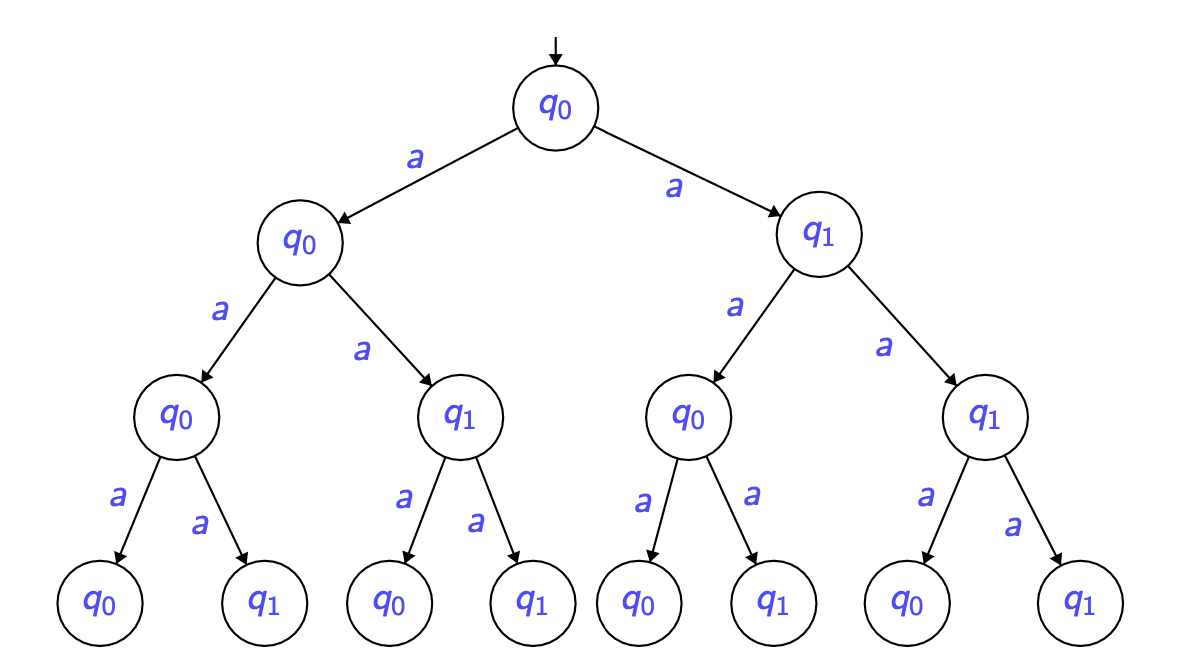
\includegraphics[scale = 0.5]{pictures/arbre_executions.png}
\end{figure}
Pour voir si un mot appartient au langage, voici ce qui sera développé :
\begin{itemize}[label=\textbullet]
    \item on va exploiter l'idée précédente pour avoir une manière efficace de tester $u \in L(A)$.
    \item Soit $P \subseteq Q$ et $\sigma \in \Sigma$. On note :
    \begin{equation*}
        \text{Post}_A(P, \sigma) = \{p | \exists p' \in P \cdot (p', \sigma, p) \in \Delta\}
    \end{equation*}
    l'ensemble des états qu'on peut atteindre à partir des états de $P$ en lisant $\sigma$.
    \item L'algorithme est le suivant :\\
        TEST(A,P,u):\\
            \indent\hspace{1cm} \textbf{case} u = epsilon :\textbf{return} P $\cap$ F $\neq \emptyset$\\
            \indent\hspace{1cm} \textbf{case} u = $\sigma$v ($\sigma\in\Sigma$) : \textbf{return} TEST(A, $Post_A(P,\sigma)$, v)
    \item $u\in L(A) \Leftrightarrow TEST(A, \{q_0\}, u)$
\end{itemize}
\begin{theorem}{Appartenance au langage non-déterministe}{app_lang_nfa}
    Étant donné un AFN $A$ avec $n$ transitions et un mot $u$ de longueur $m$, on peut tester en temps $O(|u|m)$ si $u \in L(A)$.
\end{theorem}
\begin{remark}
    Effecitvement, il suffit de remarquer dans l'algorithme que calculer $Post_A(P,\sigma)$ prend $O(m)$
\end{remark}
\begin{figure}[H]
    \centering
    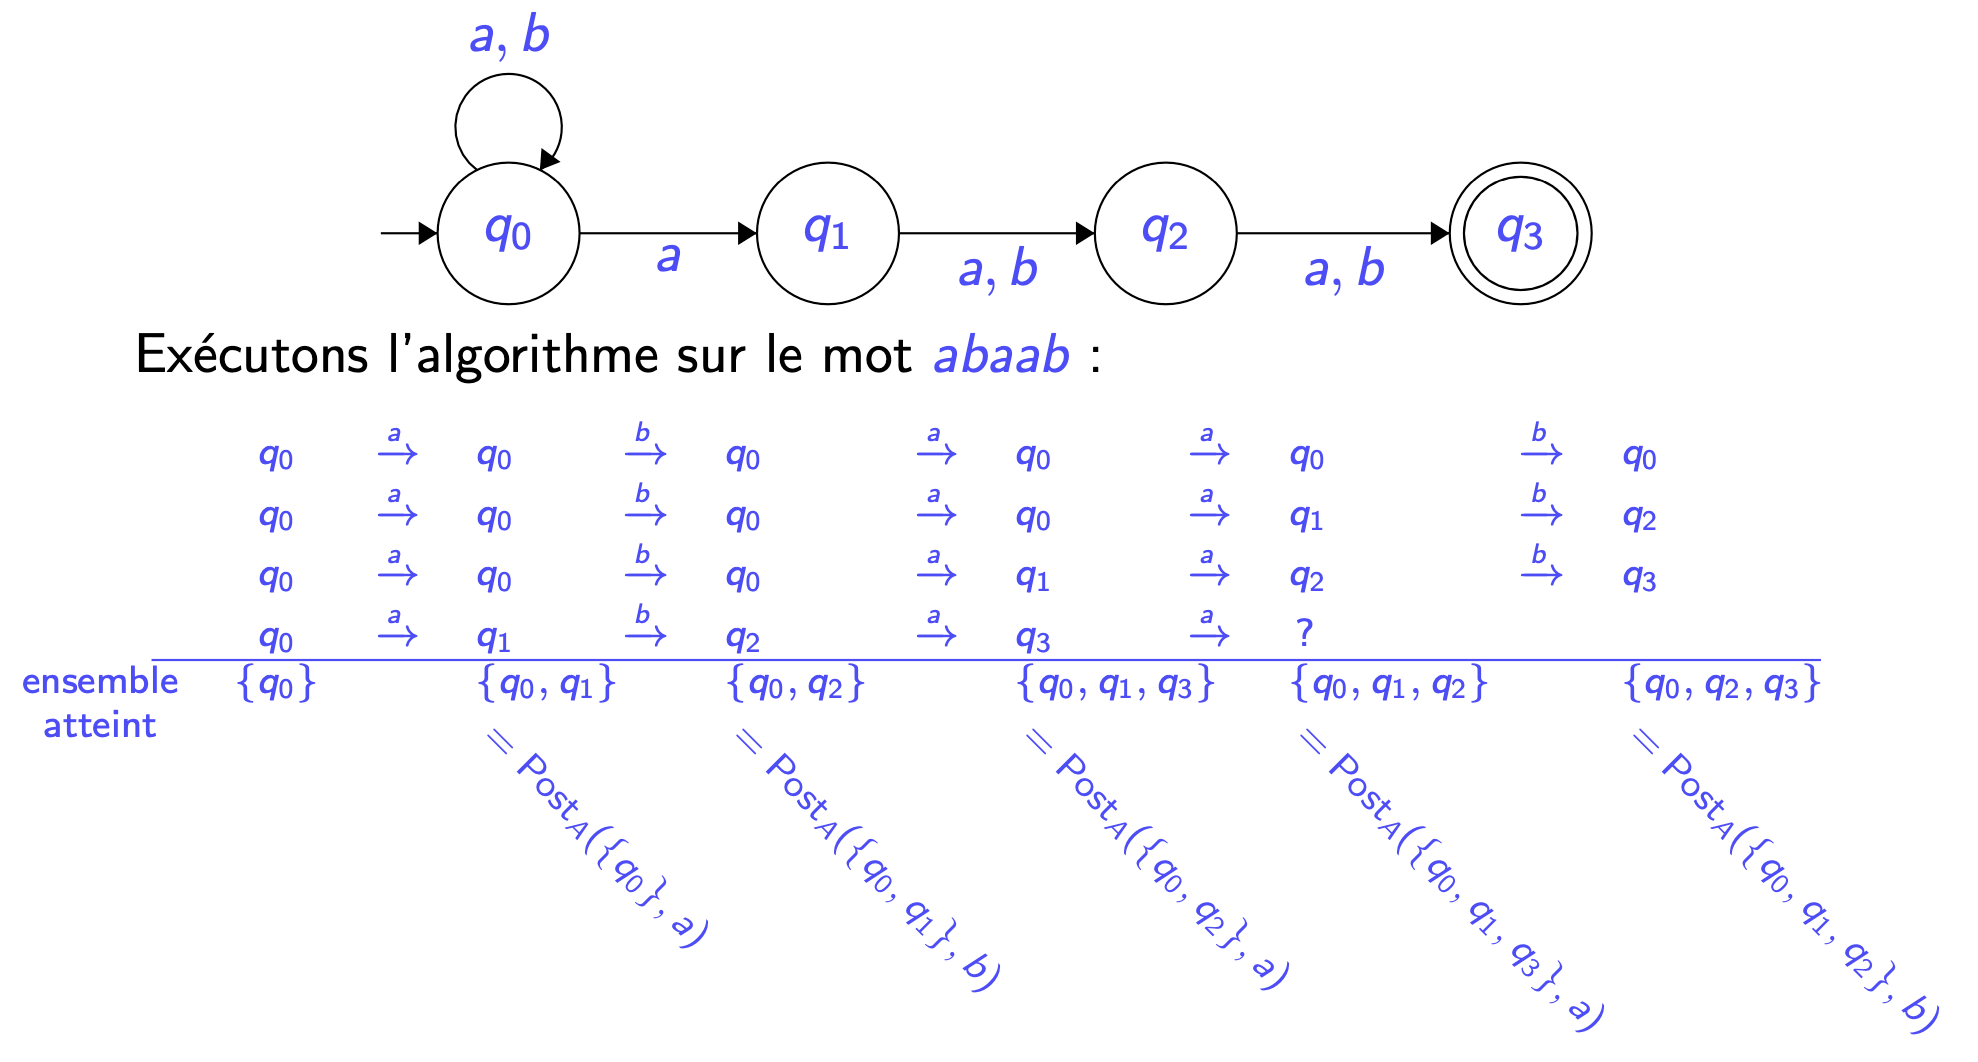
\includegraphics[scale = 0.4]{pictures/appartenance_langage_nfa.png}
\end{figure}
L'ensemble final est $\{q_0, q_1, q_2, q_3\}$ et il contient un mot acceptant et donc le mot est accepté. \\





\subsubsection{Test du vide}
\label{subsub:test_du_vide_nfa}
\begin{theorem}{Test du vide}{test_vide_nfa}
    Étant donné un AFN $A$ avec $n$ états et $m$ transitions, on peut tester en temps $O(n+m)$ si $L(A) = \emptyset$.
\end{theorem}
C'est la même chose que pour les automates déterministes.


\subsubsection{Déterminisme VS non-déterminisme}
\label{subsub:determinisme_vs_non_determinisme}

Tout langage accepté par un automate fini (déterministe) peut être accepté par un automate fini non-déterministe
 (et inversément).
\begin{theorem}{Déterminisme VS non-déterminisme}{determinisme_vs_non_determinisme}
    Soit $L$ un langage sur l'alphabet $\Sigma$. $L$ est accepté par un automate fini si et seulement s'il est accepté par un
    automate fini non-déterministe.
\end{theorem}
\begin{example}
    Voici un exemple et l'explication de cette conversion :
    \begin{itemize}[label=\textbullet]
        \item l'idée est la même que pour tester l'appartenance au langage :\\
        l'automate déterministe $B$ qui simule l'automate non-déterministe $A$ calcule le sous-ensemble d'états atteints.
        \item Les états de $B$ seront donc des sous-ensembles d'états de $A$.
        \item À partir d'un sous-ensemble $P \subseteq Q$, en lisant une lettre $\sigma$, $B$ va vers l'état $Post_A(P,\sigma)$.
        \item Les états acceptants de B sont les sous-ensembles de $Q$ qui contiennent un état final de $A$.
    \end{itemize}
    \begin{figure}[H]
        \centering
        \begin{tikzpicture} [node distance = 3cm, 
            on grid, 
            auto,
            every loop/.style={stealth-}]
        
        % State q0 
        \node (q0) [state, 
            initial, 
            initial text = {}] {$q_0$};
        
        % State q1    
        \node (q1) [state,
            right = of q0] {$q_1$};
        
        % State q2
        \node (q2) [state,
            right = of q1] {$q_2$};
        
        % State q3
        \node (q3) [state,
            accepting,
            right = of q2] {$q_3$};
        
        % Arrows
        \path [-stealth, thick]
            (q0) edge node {$a$}   (q1)
            (q0) edge [loop above]  node {$a,b$}()
            (q1) edge node {$a,b$}  (q2)
            (q2) edge node {$a,b$} (q3);
        \end{tikzpicture}
    \end{figure}
    \begin{figure}[H]
        \centering
        \begin{tikzpicture} [node distance = 3cm, 
            on grid, 
            auto,
            every loop/.style={stealth-}]
        
        % State q0 
        \node (q0) [state, 
            initial, 
            initial text = {}] {$q_0$};
        
        % State q1    
        \node (q1) [state,
            accepting,
            right = of q0] {$q_0,q_1$};

        % State q2
        \node (q2) [state,
            above right = of q1] {$q_0,q_1,q_2$};
        
        % State q3
        \node (q3) [state,
            below right = of q1] {$q_0,q_2$};
            
        % State q5
        \node (q5) [state,
            accepting,
            right = of q2] {$q_0,q_2,q_3$};
            
        % State q4
        \node (q4) [state,
            accepting,
            above = of q5] {$q_0,q_1,q_2,q_3$};
            
        % State q6
        \node (q6) [state,
            accepting,
            right = of q3] {$q_0,q_1,q_3$};
        
        % State q7
        \node (q7) [state,
            accepting,
            below = of q6] {$q_0,q_3$};

        % Arrows
        \path [-stealth, thick]
            (q0) edge node {$a$}   (q1)
            (q0) edge [loop above]  node {$b$}()
            (q1) edge node {$a$}  (q2)
            (q1) edge node {$b$}  (q3)
            (q2) edge node {$a$} (q4)
            (q2) edge node {$b$} (q5)
            (q3) edge node {$a$} (q6)
            (q3) edge node {$b$} (q7)
            (q4) edge [loop above] node {$a$}()
            (q4) edge node {$b$} (q5)
            (q5) edge node {$a$} (q6)
            (q5) edge [bend left] node {$b$} (q7)
            (q6) edge node {$a$} (q2)
            (q6) edge [bend left] node {$b$} (q3)
            (q7) edge [bend left] node {$b$} (q0)
            (q7) edge [bend left] node {$a$} (q1);
        \end{tikzpicture}
    \end{figure}
    L'automate $B$ construit a exponentiellement plus d'états que $A$. On peut montrer que $\forall n\geq 0$, le plus petit
    automate fini déterministe acceptant le langage $L_n$ des mots de longueur au moins $n$ dont la $n^{\text{ème}}$ lettre
    en partant de la fin est $a$ sur l'alphabet $\{a,b\}$, a $2^n$ états. Tandis que le plus petit AFN pour $L_n$ a $O(n)$ 
    états.
\end{example}


\subsection{Expressions rationnelles}
\label{sub:expressions_rationnelles}

\begin{definition}{Expression rationnelle}{expression_rationnelle}
    Une expression rationnelle $E$ sur un alphabet $\Sigma$ est une expresssion qui respecte la grammaire suivante :
    \begin{equation*}
        E ::= \epsilon\; |\; a\; |\; \emptyset\; |\; (E + E)\; |\; (E \cdot E)\; |\; (E^*)
    \end{equation*}
    pour tout $a \in \Sigma$.
\end{definition}
\begin{definition}{Opérations sur les langages}{op_langage}
    Soient $L,L_1,L_2\subseteq\Sigma^*$ trois langages. Alors :
    \begin{itemize}[label=\textbullet]
        \item $L_1\cdot L_2 = \{u_1 u_2 | u_1\in L_1 \wedge u_2\in L_2\}$ (noté aussi $L_1L_2$)
        \item $L^* = \{u_1,\dots,u_k | k\geq 0, u_i\in L \forall i\in \{1,\dots,k\}\}$
    \end{itemize}
\end{definition}
\begin{example}
    Voici deux exemples :
    \begin{itemize}[label=\textbullet]
        \item Si $L_1 = \{a,b\}$ et $L_2 = \{a,bb\}$ alors $L_1\cdot L_2 = \{aa,abb,ba,bbb\}$
        \item Si $L = \{a\}$ alors $L^* = \{a^n|n\geq 0\}$
    \end{itemize}
\end{example}
\begin{definition}{Sémantique des expresssions rationnelles}{sem_rati}
    La sémantique d'une expression rationnelle $E$ sur $\Sigma$ est donnée par un langage, noté $L(E)$, défini inductivement
    par :
    \begin{itemize}
        \item $L(\epsilon) = \{\epsilon\}$
        \item $L(a) = \{a\}$ pour tout $a\in\Sigma$
        \item $L(\emptyset) = \emptyset$
        \item $L(E_1 + E_2) = L(E_1) \cup L(E_2)$
        \item $L(E_1 \cdot E_2) = L(E_1) \cdot L(E_2)$
        \item $L(E^*) = L(E)^*$
    \end{itemize}
\end{definition}
\begin{example}
    Sur $\Sigma = \{a,b\}$, voici quelques exemples :
    \begin{itemize}
        \item $L((a+b)^*a(a+b)*)$ est l'ensemble des mots qui contiennent au moins un $a$.
        \item $L(a^*b^*)$ est l'ensemble des mots qui sont des séquences de $a$ suivies des séquences de $b$.
    \end{itemize}
\end{example}



\subsubsection{Expressions vers automates}
\label{subsub:expressions_vers_automates}

\begin{theorem}{Théorème de Kleene}{th_kleene}
    Tout langage est reconnaissable par un automate si et seulement s'il est définissable par une expression rationnelle.
\end{theorem}
La construction se fait par induction sur les expressions. Pour toute expression $E$, on va construire un AFN $A_E$ tel que
$L(A_E) = L(E)$ (il suffit ensuite de déterminiser $A_E$ avec la construction des sous-ensembles pour terminer la preuve).
\begin{itemize}[label=\textbullet]
    \item si $E = \epsilon$, alors $A_E = (\{q_0\}, q_0, \{q_0\}, \Delta := \emptyset)$
    \item si $E = a$, avec $a\in\Sigma$, alors $A_E = (\{q_0,q_1\}, q_0, \{q_1\}, \Delta := \{(q_0,a,q_1)\})$
    \item si $E = \emptyset$, alors $A_E = (\{q_0\}, q_0, \emptyset, \Delta := \emptyset)$
\end{itemize}


\subsubsubsection{$E=F+G$}
On construit par induction $A_F$ et $A_G$, à partir desquels on construit $A_E$ tel que :
\begin{equation*}
    L(A_E) = L(A_F) \cup L(A_G)
\end{equation*}
C'est la clôture par union (cf. Théorème \ref{clôture_union_intersection}) seulement, grâce au non-déterminisme, on peut 
faire plus simple :
\begin{itemize}[label=\textbullet]
    \item en lisant la première lettre $\sigma$, on va soit dans le premier automate soit dans le deuxième, en utilisant le
    non-déterminisme.
    \item précisément, $A_E$ a un état initial $q_0$. On note $q_0^F$ l'état initial de $A_F$ et $q_0^G$ l'état initial de
    $A_G$. Pour toute lettre $\sigma$, pour toute transition $(q_0^F,\sigma,q)\in\Delta_F$, on ajoute la transition $(q_0,
    \sigma, q)$ à $\Delta_E$. De même pour $A_G$.
    \item On rend le nouvel état initial acceptant si $q_0^F$ ou $q_0^G$ est acceptant. (pour accepter le mot vide)
\end{itemize}
\begin{figure}[H]
    \centering
    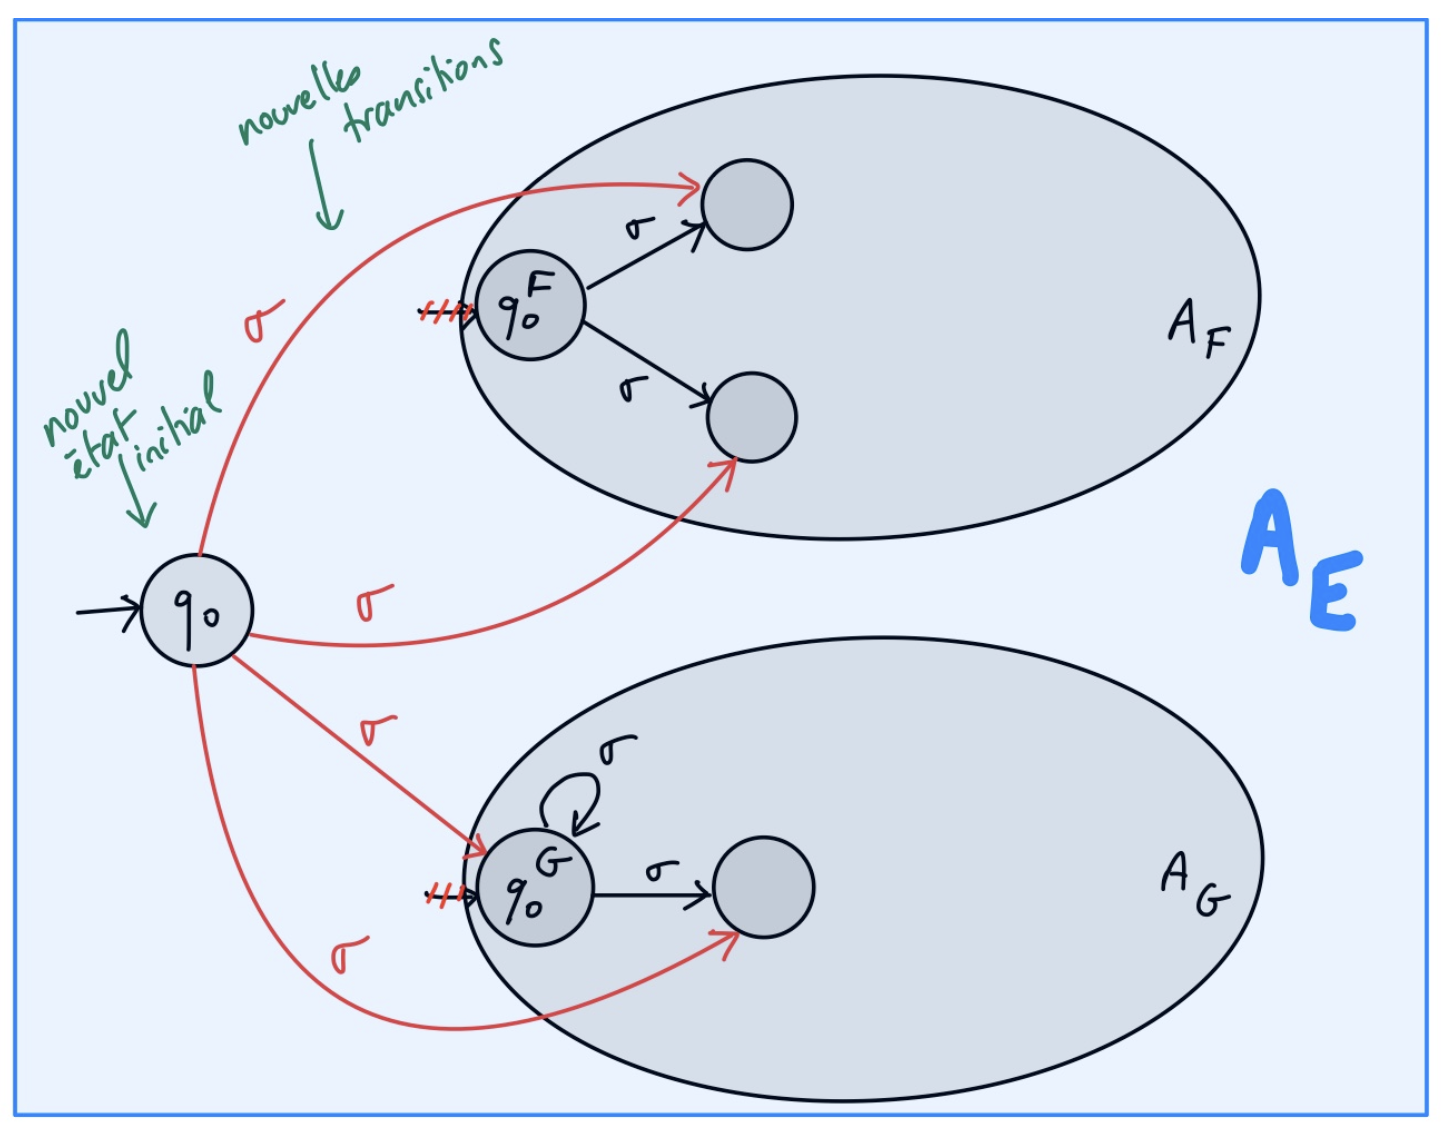
\includegraphics[scale = 0.4]{pictures/EF+G.png}
\end{figure}


\subsubsubsection{$E=FG$}
On construit $A_F$ et $A_G$ par induction, puis pour toute lettre $\sigma$, pour tout état de $A_F$ qui allait vers un état
final de $A_F$ en lisant $\sigma$, on ajoute une transition vers l'état initial de $A_G$. 
\warningbox{Les états acceptants de $A_F$ ne sont plus acceptants dans $A_E$ et l'état inital de $A_E$ est l'état initial de
$A_F$.}
\begin{figure}[H]
    \centering
    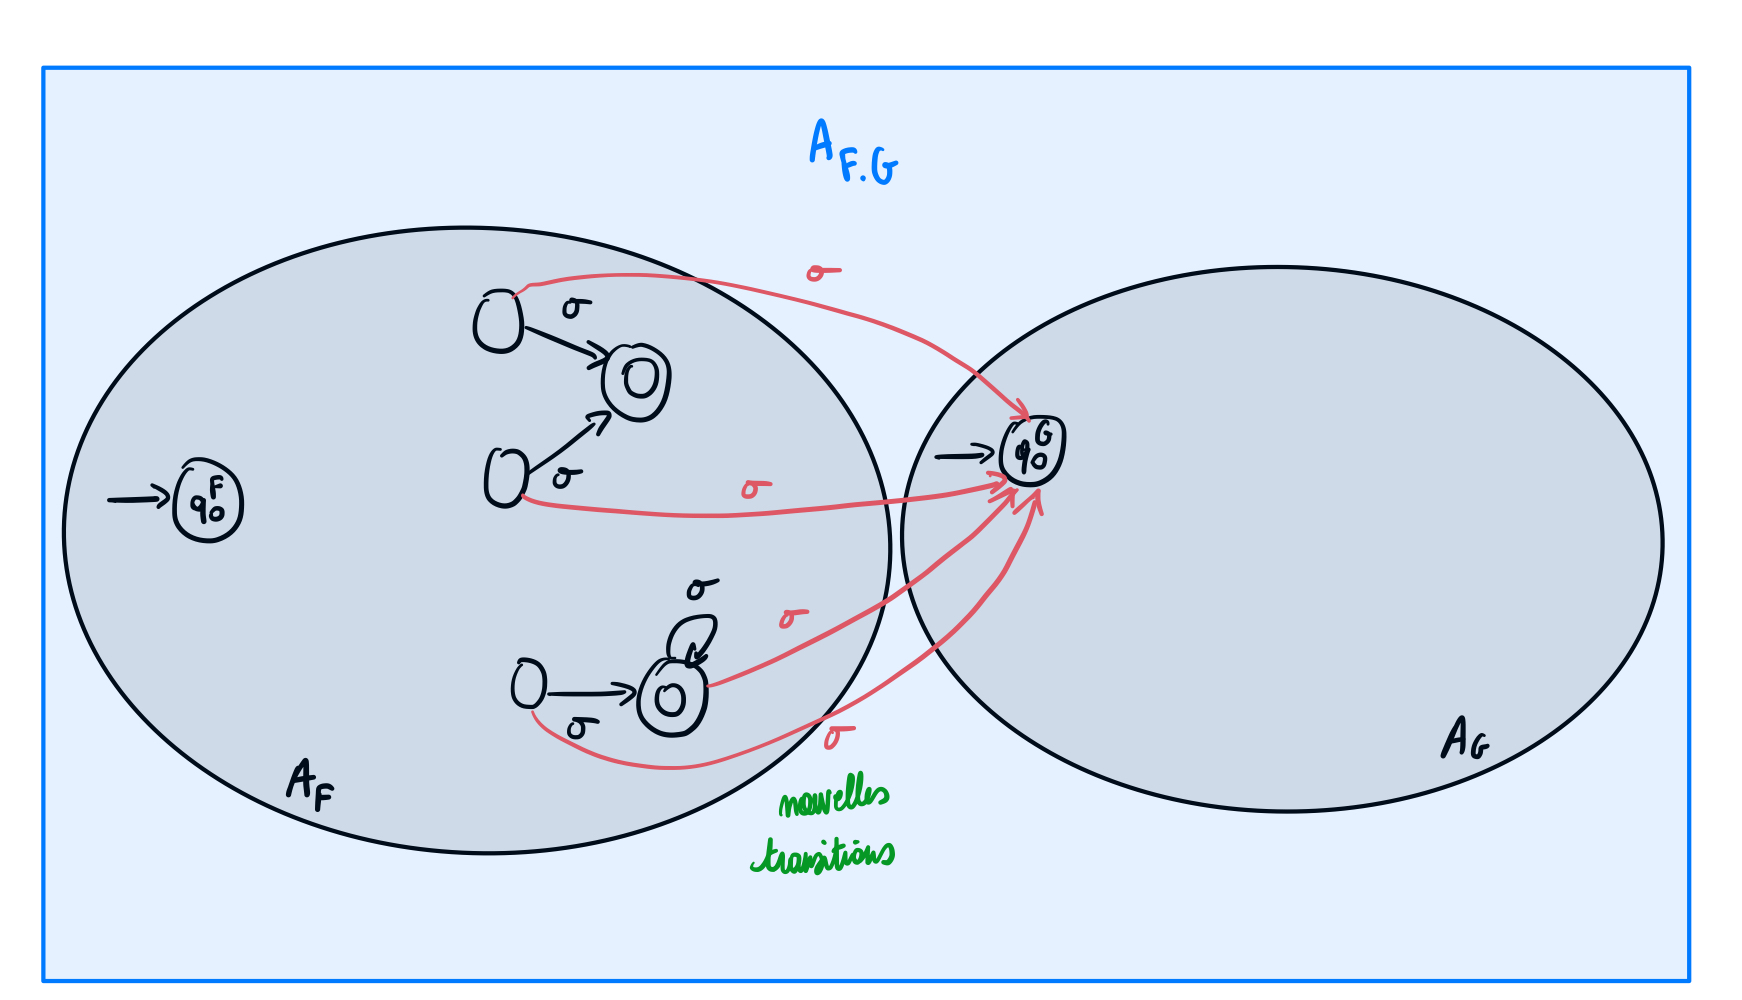
\includegraphics[scale = 0.2]{pictures/AFG.jpeg}
\end{figure}


\subsubsubsection{$E=G^*$}
Il faut faire attention au fait que $\epsilon\in L(E)$. On réécrit d'abord $E$ comme $E = \epsilon +G^+$ où $G^+$ est 
l'ensemble des mots de la forme $u_1u_2\dots u_k$ avec $k\geq 1$ et $u_i\in L(G)$ pour tout $i$.\\
Ensuite, on constrit $A_\epsilon$ et $A_G$ par induction. On montre maintenant comment obtenir $A_{G^+}$ et enfin $A_E$
sera obtenu en utilisant la clôture par union de $A_\epsilon$ et $A_{G^+}$. Pour construire $A_{G^+}$, c'est similaire à
la concaténation sauf qu'on ajoute des transitions vers l'état initial de $G$ :
\begin{figure}[H]
    \centering
    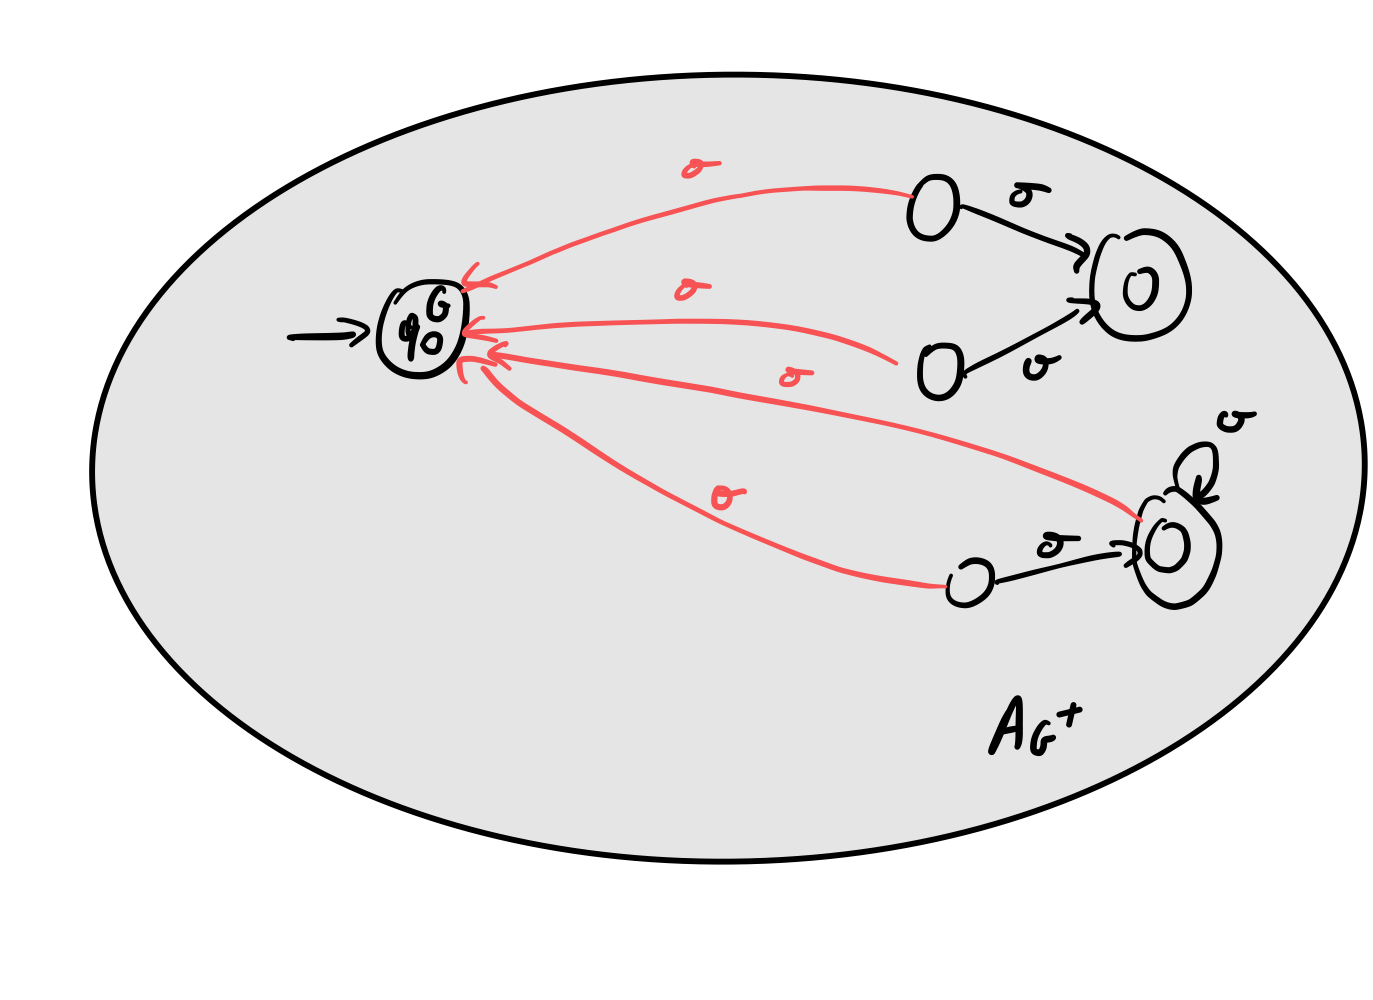
\includegraphics[scale=0.2]{pictures/AG+.jpeg}
\end{figure}


\subsection{Minimisation}
\label{sub:minimisation}

Étant donné un automate $A$, l'objectif de la minimisation est de construire un automate complet $M$ tel que $M$ a un nombre
d'états minimal et $M$ est équivalent à $A$. (cf. Définition \ref{automates_équivalents})
\begin{example}
    Voici un exemple d'un automate et de son automate minimal équivalent :
    \begin{figure}[H]
        \centering
        \begin{tikzpicture} [node distance = 3cm, 
            on grid, 
            auto,
            every loop/.style={stealth-}]
        
        % State q0 
        \node (q0) [state, 
            initial, 
            accepting, 
            initial text = {}] {$q_0$};
        
        % State q1    
        \node (q1) [state,
            accepting,
            right = of q0] {$q_1$};
        
        % Arrows
        \path [-stealth, thick]
            (q0) edge[bend left] node {$a$}   (q1)
            (q1) edge[bend left] node {$a$}   (q0)
            (q0) edge [loop above]  node {b}()
            (q1) edge [loop above]  node {b}();
        \end{tikzpicture}
    \end{figure}

    \begin{figure}[H]
        \centering
        \begin{tikzpicture} [node distance = 3cm, 
            on grid, 
            auto,
            every loop/.style={stealth-}]
        
        % State q0 
        \node (q0) [state, 
            initial, 
            accepting, 
            initial text = {}] {$q_0$};
        
        % Arrows
        \path [-stealth, thick]
            (q0) edge [loop above]  node {a,b}();
        \end{tikzpicture}
    \end{figure}
\end{example}
\begin{definition}{Sémantique}{sémantique_minimisation}
    Soit $A=(Q,q_0,F,\delta)$ un automate complet sur un alphabet $\Sigma$. Pour tout mot $u\in\Sigma^*$, pour tout état $q\in
    Q$, on note :
    \begin{itemize}[label=\textbullet]
        \item $q\cdot u$ l'état atteint à partir de $q$ en lisant $u$. (il existe car $A$ est complet)
        \item $L_q$ le langage formé des mots $u$ tels que $q\cdot u\in F$.
        \begin{equation*}
            L_q = \{u\in\Sigma^* | q\cdot u\in F\}
        \end{equation*}
        est le langage des mots acceptés à partir de $q$.
        \item pour tout $p,q\in Q, p\equiv_A q$ si $L_p = L_q$.
    \end{itemize}
\end{definition}
\begin{remark}
    $L_{q_0} = L$, $\epsilon\in L_q$ pour tout $q\in F$. $\equiv_A$ est une relation d'équivalence, on note $[p]_A$ la classe
    de tout état $p$.
\end{remark}
\noindent À partir d'un automate $A$, on calcule un automate $M_A$ comme suit :
\begin{enumerate}
    \item Il suffit de calculer toutes les classes d'équivalence de $Q$ pour $\equiv_A$, ce qui donnera les états.
    \item La classe de $q_0$ est l'état initial.
    \item Toute classe qui contient un état final est finale.
    \item On met une transition de l'état $[q]\equiv_A$ à l'état $[q\cdot a]_{\equiv_A}$ en lisant $a$, pour tout $a\in\Sigma$.
    et tout $q\in Q$.
\end{enumerate}
\begin{theorem}{Automate minimal}{automate_minimal}
    L'automate minimal $M_A$ est minimal en nombre d'états et il est l'unique automate minimal complet qui accepte $L(A)$.
\end{theorem}
\begin{example}
    Voici un exemple de calcul de l'automate minimal :
    \begin{figure}[H]
        \centering
        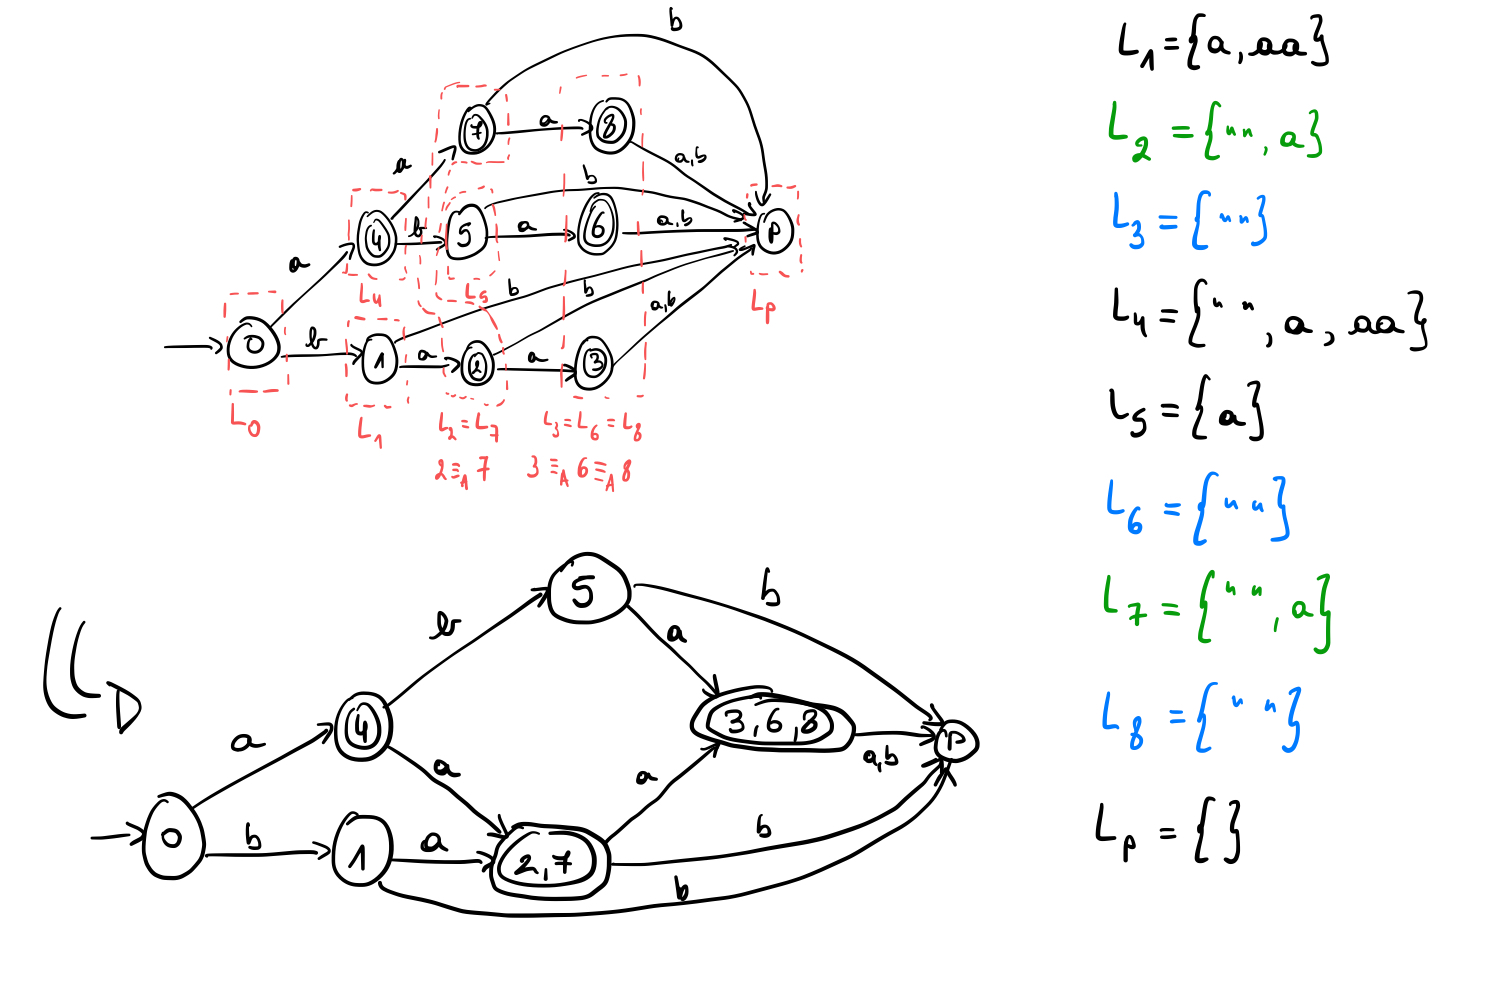
\includegraphics[scale=0.3]{pictures/automate_minimal.jpeg}
    \end{figure}
\end{example}
En pratique, ce n'est pas très efficace, on peut faire mieux, sans passer par le test d'équivalence et par raffinement 
successif de relations d'équivalence qui convergent vers $\equiv_A$. Cela est même possible en $O(n\cdot log_2(n))$ où
$n=|Q|$. Pour les AFNs, le problème d'optimisation est plus compliqué, décider si un AFN est équivalent à un AFN avec au 
plus $k$ états est PSPACE-dur.